\documentclass{book}

\usepackage{amssymb}
\usepackage{amsmath}
\usepackage{amsthm}
\usepackage{arydshln}
\usepackage{calc}
\usepackage{cancel}
\usepackage{caption}
\usepackage{cite}
\usepackage{color}
\usepackage{enumitem}
\usepackage{esint}
\usepackage{etoolbox}
\usepackage{float}
\usepackage{framed}
\usepackage{fullpage}
\usepackage{gensymb}
\usepackage[margin=1in]{geometry}
\usepackage{graphicx}
\usepackage{listings}
\usepackage{multirow}
\usepackage{subfiles}
\usepackage{rsfso}
\usepackage{tikz}
\usepackage{tikz-3dplot}
\usepackage{ushort}
\usepackage{wrapfig}
\usepackage{xcolor}
\usepackage{soul}
\usepackage{epstopdf}

% pdf versions
\pdfoptionpdfminorversion=7

% handle page stretching
\raggedbottom

% Graphics file location
\graphicspath{{Graphics/}{../Graphics/}}

% Use for drawings
\usetikzlibrary{angles,arrows,calc,decorations,intersections,patterns,positioning,quotes,shapes}
\usetikzlibrary{shapes.geometric}
\usetikzlibrary{decorations.pathreplacing}
\newcommand{\midarrow}{\tikz \draw[-latex] (0,0) -- +(.1,0);}

% Tikz commands for drawing block diagrams, etc...
\tikzset{%
	block/.style    = {draw, rectangle, minimum height = 2em, minimum width = 2em},
	sum/.style      = {draw, circle}, % Adder
	input/.style    = {fill=white, rectangle}, % Input
	output/.style   = {fill=white, rectangle}, % Output
	waypoint/.style   = {coordinate}, % Output
}

\tikzset{%
	startstop/.style= {draw, rectangle, rounded corners, minimum width=2cm, minimum height=1cm,text centered},
	inout/.style    = {draw, trapezium, trapezium left angle=70, trapezium right angle=110, minimum width=2cm, minimum height=1cm, text centered},
	process/.style  = {draw, rectangle, minimum width=2cm, minimum height=1cm, text centered},
	decision/.style = {draw, diamond, minimum width=1.5cm, minimum height=1cm, text centered, diamond, aspect=2},
	arrow/.style    = {thick,-latex,>=stealth},		
}

\tikzset{
	saveuse path/.code 2 args={
		\pgfkeysalso{#1/.style={insert path={#2}}}%
		\global\expandafter\let\csname pgfk@\pgfkeyscurrentpath/.@cmd\expandafter\endcsname
		% not optimal as it is now global through out the document
		\csname pgfk@\pgfkeyscurrentpath/.@cmd\endcsname
		\pgfkeysalso{#1}},
	/pgf/math set seed/.code=\pgfmathsetseed{#1}}

% Define Laplace, Fourier transform symbols
\newcommand{\LT}{\mathcal{L}}
\newcommand{\FT}{\mathcal{F}}

% Define adjugate function
\newcommand{\adj}{\text{adj}}

% Define rank function
\newcommand{\rank}{\text{rank}}

% commands to speed up writing j\omega and s-plane
\newcommand{\jw}{j\omega}
\newcommand{\jt}{j\theta}
\newcommand{\wt}{\omega t}
\newcommand{\zw}{\zeta\omega_n}
\newcommand{\spl}{s\textrm{-plane}}
\newcommand{\Lm}{\textrm{Lm }}
% Clean up overline/underline for math mode
\def\obar#1{\bar{#1}}
\def\ubar#1{\ushort{#1}}

\newcommand{\exmp}{\subsubsection*{Example}}
\newcommand{\nib}{\noindent$ \bullet\ $}


\begin{document}
\chapter*{Lecture 8}
Last time: Reviewed Stability
\begin{itemize}
	\item Stability requirements
	\item Routh-Hurwitz Criterion
\end{itemize}
Last lecture, we mentioned that we have not yet addressed the issue of accuracy of the final value of a system's output, in other words how close a system's final value is to the desired value. This lecture we will learn about block diagram algebra, which is a tool we will use to assess steady-state error in the next lecture.

\section*{Block Diagram Reduction}
Block Diagrams are used quite a bit in the study of control systems --- mainly in their representation. Sometimes, we are interested in reducing a relatively complex block diagram system to a simpler form. 

\exmp
\begin{center}
	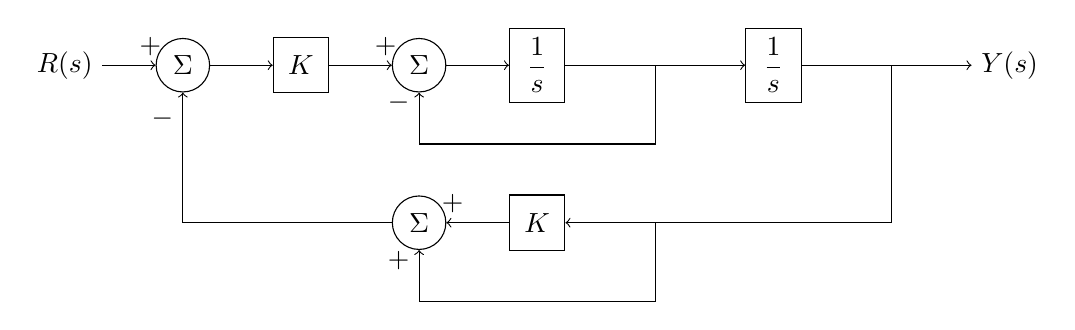
\begin{tikzpicture}[node distance = 1.5cm]
	\node[input] (r) {$ R(s) $};
	\node[sum,right of=r] (sum1) {$ \Sigma $};
	\node[block,right of=sum1] (K1) {$ K $};
	\node[sum,right of=K1] (sum2) {$ \Sigma $};
	\node[block,right of=sum2] (s1) {$ \dfrac{1}{s}$};
	\node[waypoint,right of=s1] (wp1) {};
	\node[block,right of=wp1] (s2) {$ \dfrac{1}{s}$};
	\node[waypoint,right of=s2] (wp2) {};
	\node[output,right of=wp2] (y) {$ Y(s) $};
	\node[waypoint,below of=s1,node distance = 1cm] (wp3) {};
	\node[block,below of=wp3,node distance = 1cm] (K2) {$ K $};
	\node[waypoint,right of=K2] (wp4) {};
	\node[sum,left of=K2] (sum3) {$ \Sigma $};
	\node[waypoint,below of=K2,node distance = 1cm] (wp5) {};
	
	\draw[->] (r) -- node[pos=0.9,above] {$ + $} (sum1);
	\draw[->] (sum1) -- (K1);
	\draw[->] (K1) -- node[pos=0.9,above] {$ + $} (sum2);
	\draw[->] (sum2) -- (s1);
	\draw[->] (s1) -- (s2);
	\draw[->] (wp1) |- (wp3) -| node[pos=0.9,left] {$ - $} (sum2);
	\draw[->] (s2) -- (y);
	\draw[->] (wp2) |- (K2);
	\draw[->] (K2) -- node[pos=0.9,above] {$ + $} (sum3);
	\draw[->] (wp4) |- (wp5) -| node[pos=0.9,left] {$ + $} (sum3);
	\draw[->] (sum3) -| node[pos=0.9,left] {$ - $}  (sum1);
	\end{tikzpicture}
\end{center}
How can we reduce this to
\begin{center}
	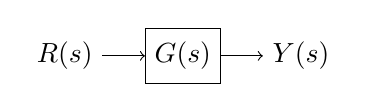
\begin{tikzpicture}[node distance = 1.5cm]
	\node[input] (r) {$ R(s) $};
	\node[block,right of=r] (G) {$ G(s)$};
	\node[output,right of=G] (y) {$ Y(s) $};
	\draw[->] (r) -- (G);
	\draw[->] (G) -- (y);
	\end{tikzpicture}
\end{center}
How do we find $ G(s) $?

\subsection*{Basic Elements}
First, let's consider two basic elements that occur when several subsystems are connected together:
\begin{itemize}
	\item The summing junction
	\item The pick-off point
\end{itemize}
\subsubsection*{The summing junction}
\begin{center}
	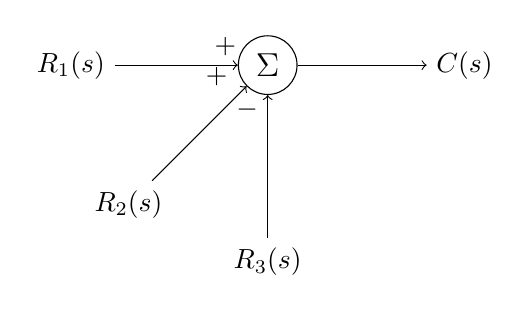
\begin{tikzpicture}[node distance = 2.5cm]
	\node[input] (r) {$ R_1(s) $};
	\node[sum,right of=r] (sum) {\large$ \Sigma $};		
	\node[input,below of=sum] (r2) {$ R_3(s) $};
	\node[input,below left of=sum] (r3) {$ R_2(s) $};
	\node[output,right of=sum] (y) {$ C(s) $};
	\draw[->] (r) -- node[pos=0.9,above] {$+$} (sum);
	\draw[->] (r2) -- node[pos=0.9,left] {$-$} (sum);
	\draw[->] (r3) -- node[pos=0.9,above left] {$+$} (sum);
	\draw[->] (sum) -- (y);
	\end{tikzpicture}
\end{center}
$ C(s) $ is the algebraic sum of all the signals going into the junction.
\[ C(s) = R_1(s) + R_2(s) - R_3(s) \]

\subsubsection*{The pick-off point}
\begin{center}
	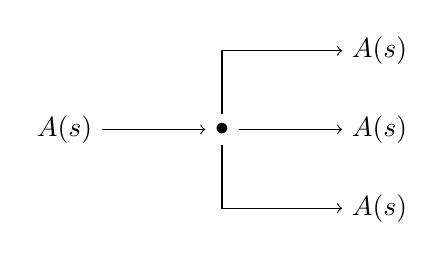
\begin{tikzpicture}[node distance = 2cm]
	\node[input] (r) {$ A(s) $};
	\node[right of=r] (sum) {$ \bullet $};		
	\node[output,right of=sum] (y) {$ A(s) $};
	\node[output,above of=y,node distance = 1cm] (y2) {$ A(s) $};
	\node[output,below of=y,node distance = 1cm] (y3) {$ A(s) $};
	\draw[->] (r) -- (sum);
	\draw[->] (sum) -- (y);
	\draw[->] (sum) |- (y2);
	\draw[->] (sum) |- (y3);
	\end{tikzpicture}
\end{center}
The pickoff point distributes the input signal undiminished to all its output points.

\subsection*{Common Interconnection Topologies}
Now, lets look at some common topologies, and solve them using our knowledge of the basic elements.
\subsubsection{1. The Cascade Form}
\begin{center}
	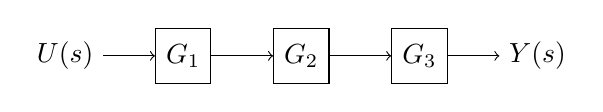
\begin{tikzpicture}[node distance = 1.5cm]
	\node[input] (r) {$ U(s) $};
	\node[block,right of=r] (G1) {$ G_1 $};
	\node[block,right of=G1] (G2) {$ G_2 $};
	\node[block,right of=G2] (G3) {$ G_3 $};
	\node[output,right of=G3] (y) {$ Y(s) $};
	\draw[->] (r) -- (G1);
	\draw[->] (G1) -- (G2);
	\draw[->] (G2) -- (G3);
	\draw[->] (G3) -- (y);
	\end{tikzpicture}
\end{center}
We have seen that, in the Laplace domain, the output of a block equals the input times the transfer function.
\begin{center}
	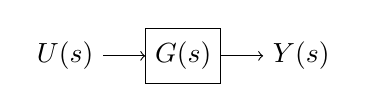
\begin{tikzpicture}[node distance = 1.5cm]
	\node[input] (r) {$ U(s) $};
	\node[block,right of=r] (G) {$ G(s)$};
	\node[output,right of=G] (y) {$ Y(s) $};
	\draw[->] (r) -- (G);
	\draw[->] (G) -- (y);
	\end{tikzpicture}
	\[ Y(s) = G(s) U(s) \]
\end{center} 
If we have multiple blocks \textbf{in cascade},
\begin{center}
	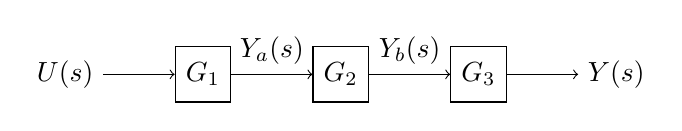
\begin{tikzpicture}[node distance = 1.75cm]
	\node[input] (r) {$ U(s) $};
	\node[block,right of=r] (G1) {$ G_1 $};
	\node[block,right of=G1] (G2) {$ G_2 $};
	\node[block,right of=G2] (G3) {$ G_3 $};
	\node[output,right of=G3] (y) {$ Y(s) $};
	\draw[->] (r) -- (G1);
	\draw[->] (G1) -- node[above] {$ Y_a(s) $} (G2);
	\draw[->] (G2) -- node[above] {$ Y_b(s) $} (G3);
	\draw[->] (G3) -- (y);
	\end{tikzpicture}
\end{center}
So, we have
\begin{align*}
Y(s) & = G_3(s)Y_b(s)\\
& = G_3(s) G_2(s) Y_a(s)\\
& = G_3(s) G_2(s) G_1(s) U(s)\\
G(s) = G_1G_2G_3
\end{align*}

\subsubsection{2. The Feedback Form}
We have seen that a typical feedback control system has the schematic form
\begin{center}
	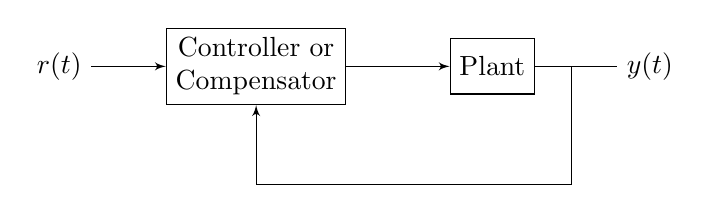
\begin{tikzpicture}[node distance=2.0cm,auto,>=latex']
	\node [input,align=center] (r) {$r(t)$};
	\node [block,align=center] (sumr) [right of=r,node distance=2.5cm] {Controller or\\Compensator};
	\node [block] (gp) [right of=sumr,node distance=3.0cm] {Plant};
	\node [waypoint] (wp) [right of=gp,node distance=1.0cm] {Sensor};
	\node [output,align=center] (y) [right of=gp,node distance=2cm]{$y(t)$};
	\node [waypoint] (h) [below of=gp,node distance=1.5cm] {Sensor};
	
	\draw[->] (r) --  (sumr);
	\draw[->] (sumr) -- (gp);
	\draw (gp) -- (y);
	\draw[->] (wp) |- (h) -| (sumr);
	
	\end{tikzpicture}
\end{center}
In block diagram form (in the Laplace domain), we have:
\begin{center}
	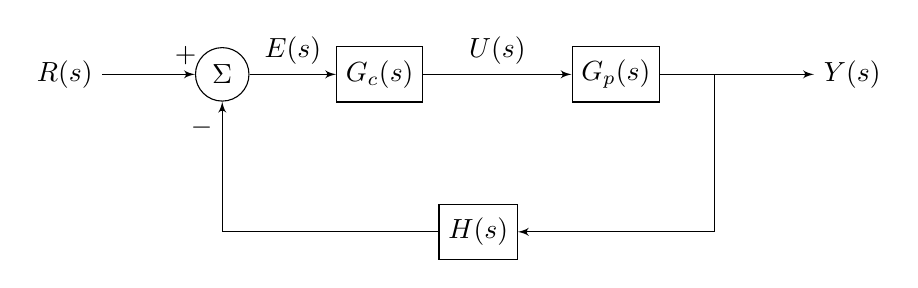
\begin{tikzpicture}[node distance=2.0cm,auto,>=latex']
	\node [input,align=center] (r) {$ R(s) $};
	\node [sum] (sumr) [right of=r] {$\Sigma$};
	\node [block] (gc) [right of=sumr] {$ G_c(s) $};
	\node [block] (gp) [right of=gc,node distance=3.0cm] {$ G_p(s) $};
	\node [waypoint] (sumd) [right of=gp,node distance=1.25cm] {};
	\node [output,align=center] (y) [right of=sumd,node distance=1.75cm]{$ Y(s) $};
	\node [waypoint] (sumn) [below of=sumd] {};
	\node [block] (h) [left of=sumn,node distance=3cm] {$ H(s) $};
	
	\draw[->] (r) -- node[pos=0.9] {$+$} (sumr);
	\draw[->] (sumr) -- node {$E(s)$} (gc);
	\draw[->] (gc) -- node {$U(s)$} (gp);
	\draw (gp) -- (sumd);
	\draw (sumd) -- (sumn);
	\draw[->] (sumd) -- (y);
	\draw[->] (sumn) -- (h);
	\draw[->] (h) -| node[pos=0.9] {$-$} (sumr);	
	\end{tikzpicture}
\end{center}
and we want:
\begin{center}
	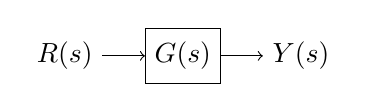
\begin{tikzpicture}[node distance = 1.5cm]
	\node[input] (r) {$ R(s) $};
	\node[block,right of=r] (G) {$ G(s)$};
	\node[output,right of=G] (y) {$ Y(s) $};
	\draw[->] (r) -- (G);
	\draw[->] (G) -- (y);
	\end{tikzpicture}
\end{center}
where $ G(s) $ is such that $ Y(s) = G(s)U(s) $. From the block diagram:
\begin{align*}
Y(s) & = G_p(s)U(s)\\
U(s) & = G_c(s)E(s)\\
E(s) & = R(s) - H(s) Y(s)\\
\end{align*}
So,
\[ Y(s) = G_pU(s) = G_pG_c E(s) = G_pG_c(R(s) - HY(s)) \]
or,
\[ Y(s) = G_pG_c R(s) - G_pG_cHY(s) \]
then,
\[ (1+G_cG_pH)Y(s) = G_cG_pR(s) \]
\[ \boxed{\frac{Y}{R}(s) = \frac{G_cG_p}{1+G_cG_pH} = G(s)} \]
We define $ L(s) $ as
\[ L(s) = G_cG_pH \]
called the return ratio, loop gain, loop transmission, or open-loop transfer function. In general:
\[ \frac{output}{input} = \frac{direct\ path}{1+return\ ratio} \]
This is true for simple closed-loop systems with negative feedback.

\exmp
\begin{center}
	\begin{tikzpicture}[node distance=2.0cm,auto,>=latex']
	\node [input,align=center] (r) {$ R(s) $};
	\node [sum] (sumr) [right of=r] {$\Sigma$};
	\node [block] (gc) [right of=sumr] {$ K $};
	\node [block] (gp) [right of=gc,node distance=3.0cm] {$ \dfrac{1}{s(s+2)} $};
	\node [waypoint] (sumd) [right of=gp,node distance=1.25cm] {};
	\node [output,align=center] (y) [right of=sumd,node distance=1.75cm]{$ Y(s) $};
	\node [waypoint] (sumn) [below of=sumd] {};
	\node [waypoint] (h) [left of=sumn,node distance=3cm] {$ H(s) $};
	
	\draw[->] (r) -- node[pos=0.9] {$+$} (sumr);
	\draw[->] (sumr) -- (gc);
	\draw[->] (gc) -- (gp);
	\draw (gp) -- (sumd);
	\draw (sumd) -- (sumn);
	\draw[->] (sumd) -- (y);
	\draw[->] (sumn) -- (h) -| node[pos=0.9] {$-$} (sumr);	
	\end{tikzpicture}
\end{center}
\[ \frac{Y}{R}(s) = \frac{K\dfrac{1}{s(s+2)}}{1+K\dfrac{1}{s(s+2)}} = \dfrac{K}{s(s+2)+K} \]
\[ \frac{Y}{R}(s) = \dfrac{K}{s^2+2s+K} \]
\begin{center}
	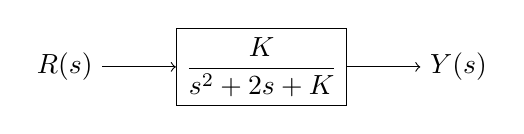
\begin{tikzpicture}[node distance = 2.5cm]
	\node[input] (r) {$ R(s) $};
	\node[block,right of=r] (G) {$ \dfrac{K}{s^2+2s+K}$};
	\node[output,right of=G] (y) {$ Y(s) $};
	\draw[->] (r) -- (G);
	\draw[->] (G) -- (y);
	\end{tikzpicture}
\end{center}

\subsubsection{3. The Parallel Form}
\begin{center}
	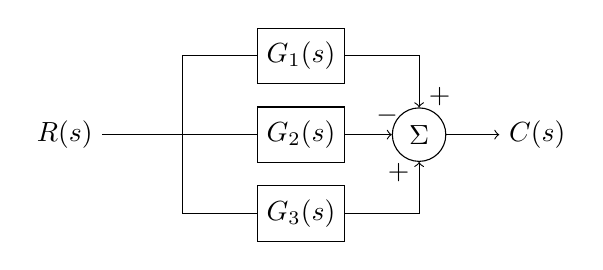
\begin{tikzpicture}[node distance = 1.5cm]
	\node[input] (r) {$ R(s) $};
	\node[waypoint,right of=r] (pop) {$ \bullet $};		
	\node[block,right of=pop] (wp1) {$ G_2(s) $};
	\node[block,above of=wp1,node distance = 1cm] (wp2) {$ G_1(s) $};
	\node[block,below of=wp1,node distance = 1cm] (wp3) {$ G_3(s) $};
	\node[sum,right of=wp1] (sum) {$ \Sigma $};	
	\node[output,right of=sum] (y) {$ C(s) $};
	\draw[->] (r) -- (wp1) -- node[pos=0.9,above] {$ - $} (sum);
	\draw[->] (pop) |- (wp2) -| node[pos=0.9,right] {$ + $} (sum);
	\draw[->] (pop) |- (wp3) -| node[pos=0.9,left] {$ + $} (sum);
	\draw[->] (sum) -- (y);
	\end{tikzpicture}
\end{center}
Using our knowledge of pickoff points and summing junctions,
\[ C(s) = G_1(s)R(s) - G_2(s)R(s) + G_3(s)R(s) \]
\[ C(s) = \left(G_1(s)-G_2(s)+G_3(s)\right)R(s) \]
\begin{center}
	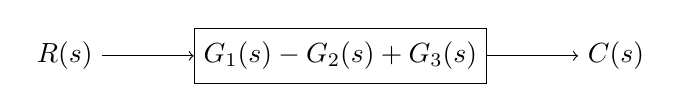
\begin{tikzpicture}[node distance = 3.5cm]
	\node[input] (r) {$ R(s) $};
	\node[block,right of=r] (G) {$ G_1(s)-G_2(s)+G_3(s)$};
	\node[output,right of=G] (y) {$ C(s) $};
	\draw[->] (r) -- (G);
	\draw[->] (G) -- (y);
	\end{tikzpicture}
\end{center}

\exmp
\begin{center}
	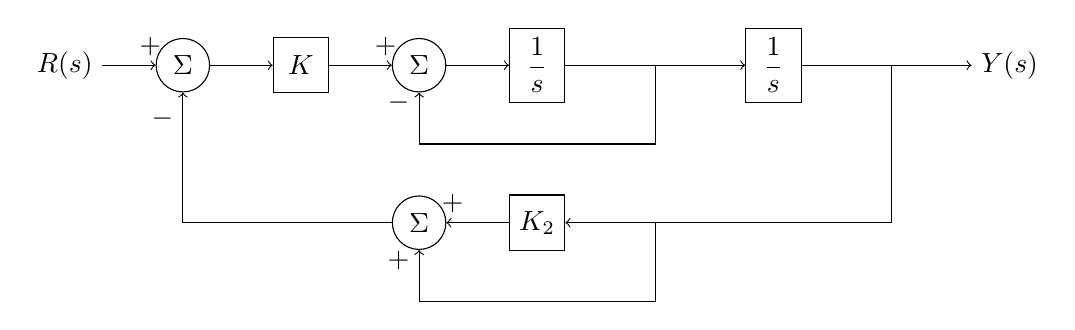
\begin{tikzpicture}[node distance = 1.5cm]
	\node[input] (r) {$ R(s) $};
	\node[sum,right of=r] (sum1) {$ \Sigma $};
	\node[block,right of=sum1] (K1) {$ K $};
	\node[sum,right of=K1] (sum2) {$ \Sigma $};
	\node[block,right of=sum2] (s1) {$ \dfrac{1}{s}$};
	\node[waypoint,right of=s1] (wp1) {};
	\node[block,right of=wp1] (s2) {$ \dfrac{1}{s}$};
	\node[waypoint,right of=s2] (wp2) {};
	\node[output,right of=wp2] (y) {$ Y(s) $};
	\node[waypoint,below of=s1,node distance = 1cm] (wp3) {};
	\node[block,below of=wp3,node distance = 1cm] (K2) {$ K_2 $};
	\node[waypoint,right of=K2] (wp4) {};
	\node[sum,left of=K2] (sum3) {$ \Sigma $};
	\node[waypoint,below of=K2,node distance = 1cm] (wp5) {};
	
	\draw[->] (r) -- node[pos=0.9,above] {$ + $} (sum1);
	\draw[->] (sum1) -- (K1);
	\draw[->] (K1) -- node[pos=0.9,above] {$ + $} (sum2);
	\draw[->] (sum2) -- (s1);
	\draw[->] (s1) -- (s2);
	\draw[->] (wp1) |- (wp3) -| node[pos=0.9,left] {$ - $} (sum2);
	\draw[->] (s2) -- (y);
	\draw[->] (wp2) |- (K2);
	\draw[->] (K2) -- node[pos=0.9,above] {$ + $} (sum3);
	\draw[->] (wp4) |- (wp5) -| node[pos=0.9,left] {$ + $} (sum3);
	\draw[->] (sum3) -| node[pos=0.9,left] {$ - $}  (sum1);
	\end{tikzpicture}
\end{center}
Reduce the inner feedback loop and bottom parallel form.
\begin{center}
	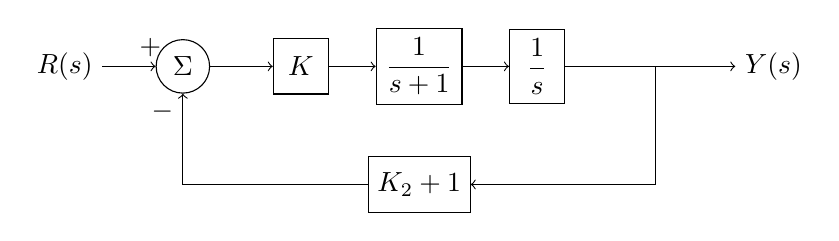
\begin{tikzpicture}[node distance = 1.5cm]
	\node[input] (r) {$ R(s) $};
	\node[sum,right of=r] (sum1) {$ \Sigma $};
	\node[block,right of=sum1] (K1) {$ K $};
	\node[block,right of=K1] (s1) {$ \dfrac{1}{s+1}$};
	\node[block,right of=s1] (s2) {$ \dfrac{1}{s}$};
	\node[waypoint,right of=s2] (wp2) {};
	\node[output,right of=wp2] (y) {$ Y(s) $};
	\node[block,below of=s1,node distance = 1.5cm] (K2) {$ K_2+1 $};
	
	\draw[->] (r) -- node[pos=0.9,above] {$ + $} (sum1);
	\draw[->] (sum1) -- (K1);
	\draw[->] (K1) -- (s1);
	\draw[->] (s1) -- (s2);
	\draw[->] (s2) -- (y);
	\draw[->] (wp2) |- (K2);
	\draw[->] (K2) -| node[pos=0.9,left] {$ - $}  (sum1);
	\end{tikzpicture}
\end{center}
Reduce the cascading form.
\begin{center}
	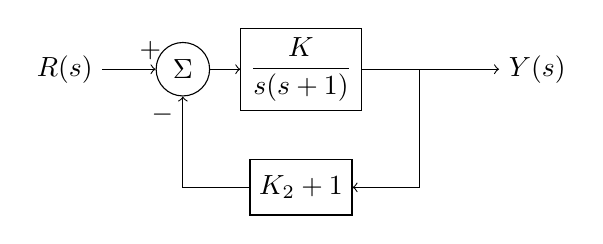
\begin{tikzpicture}[node distance = 1.5cm]
	\node[input] (r) {$ R(s) $};
	\node[sum,right of=r] (sum1) {$ \Sigma $};
	\node[block,right of=sum1] (s1) {$ \dfrac{K}{s(s+1)} $};
	\node[waypoint,right of=s1] (wp2) {};
	\node[output,right of=wp2] (y) {$ Y(s) $};
	\node[block,below of=s1,node distance = 1.5cm] (K2) {$ K_2+1 $};
	
	\draw[->] (r) -- node[pos=0.9,above] {$ + $} (sum1);
	\draw[->] (sum1) -- (s1);
	\draw[->] (s1) -- (y);
	\draw[->] (wp2) |- (K2);
	\draw[->] (K2) -| node[pos=0.9,left] {$ - $}  (sum1);
	\end{tikzpicture}
\end{center}
Condense the feedback loop.
\begin{center}
	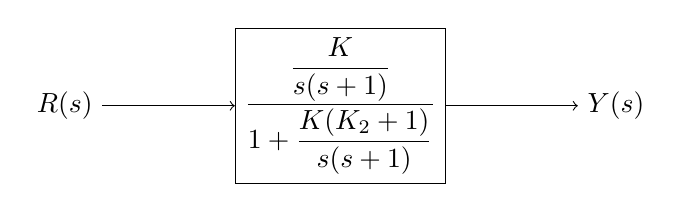
\begin{tikzpicture}[node distance = 3.5cm]
	\node[input] (r) {$ R(s) $};
	\node[block,right of=r] (G) {$ \dfrac{\dfrac{K}{s(s+1)}}{1+\dfrac{K(K_2+1)}{s(s+1)}}$};
	\node[output,right of=G] (y) {$ Y(s) $};
	\draw[->] (r) -- (G);
	\draw[->] (G) -- (y);
	\end{tikzpicture}
\end{center}
Simplify the transfer function.
\begin{center}
	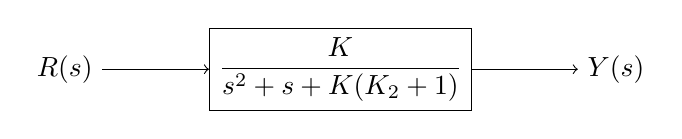
\begin{tikzpicture}[node distance = 3.5cm]
	\node[input] (r) {$ R(s) $};
	\node[block,right of=r] (G) {$ \dfrac{K}{s^2+s+{K}({K_2+1})}$};
	\node[output,right of=G] (y) {$ Y(s) $};
	\draw[->] (r) -- (G);
	\draw[->] (G) -- (y);
	\end{tikzpicture}
\end{center}

\exmp
\begin{center}
	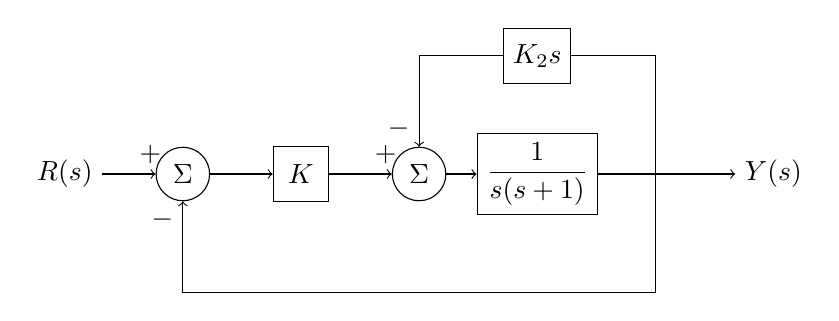
\begin{tikzpicture}[node distance = 1.5cm]
	\node[input] (r) {$ R(s) $};
	\node[sum,right of=r] (sum1) {$ \Sigma $};
	\node[block,right of=sum1] (K1) {$ K $};
	\node[sum,right of=K1] (sum2) {$ \Sigma $};
	\node[block,right of=sum2] (s1) {$ \dfrac{1}{s(s+1)}$};
	\node[waypoint,right of=s1] (wp1) {};
	\node[block,above of=s1] (s2) {$ K_2 s $};
	\node[waypoint,right of=s1] (wp2) {};
	\node[output,right of=wp1] (y) {$ Y(s) $};
	\node[waypoint,below of=sum2] (wpb) {};
	
	\draw[->] (r) -- node[pos=0.9,above] {$ + $} (sum1);
	\draw[->] (sum1) -- (K1);
	\draw[->] (K1) -- node[pos=0.9,above] {$ + $} (sum2);
	\draw[->] (sum2) -- (s1);
	\draw[->] (s1) -- (y);
	\draw[->] (wp1) |- (s2) -| node[pos=0.9,left] {$ - $} (sum2);
	\draw[->] (wp1) |- (wpb) -| node[pos=0.9,left] {$ - $}  (sum1);
	\end{tikzpicture}
\end{center}
Rearrange (split the pickoff point apart).
\begin{center}
	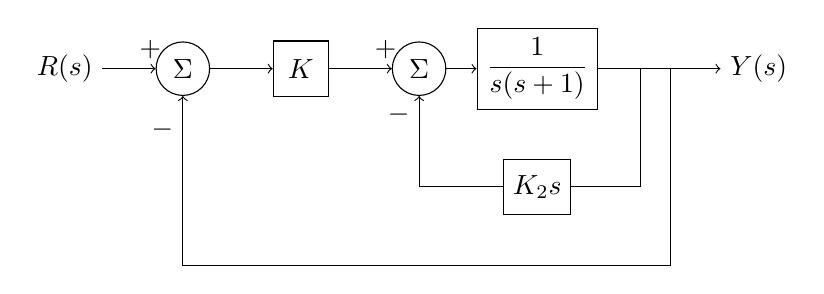
\begin{tikzpicture}[node distance = 1.5cm]
	\node[input] (r) {$ R(s) $};
	\node[sum,right of=r] (sum1) {$ \Sigma $};
	\node[block,right of=sum1] (K1) {$ K $};
	\node[sum,right of=K1] (sum2) {$ \Sigma $};
	\node[block,right of=sum2] (s1) {$ \dfrac{1}{s(s+1)}$};
	\node[waypoint,right of=s1,node distance = 1.3125cm] (wp1) {};
	\node[block,below of=s1] (s2) {$ K_2 s $};
	\node[waypoint,right of=s1,node distance = 1.6875cm] (wp2) {};
	\node[output,right of=wp1] (y) {$ Y(s) $};
	\node[waypoint,below of=sum2,node distance = 2.5cm] (wpb) {};
	
	\draw[->] (r) -- node[pos=0.9,above] {$ + $} (sum1);
	\draw[->] (sum1) -- (K1);
	\draw[->] (K1) -- node[pos=0.9,above] {$ + $} (sum2);
	\draw[->] (sum2) -- (s1);
	\draw[->] (s1) -- (y);
	\draw[->] (wp1) |- (s2) -| node[pos=0.9,left] {$ - $} (sum2);
	\draw[->] (wp2) |- (wpb) -| node[pos=0.9,left] {$ - $}  (sum1);
	\end{tikzpicture}
\end{center}
Condense the feedback loop.
\begin{center}
	\begin{tikzpicture}[node distance = 1.5cm]
	\node[input] (r) {$ R(s) $};
	\node[sum,right of=r] (sum1) {$ \Sigma $};
	\node[block,right of=sum1] (K1) {$ K $};
	\node[block,right of=K1,node distance = 2.5cm] (s1) {$ \dfrac{\dfrac{1}{s(s+1)}}{1+\dfrac{K_2s}{s(s+1)}} $};
	\node[waypoint,right of=s1,node distance = 2.5cm] (wp1) {};
	\node[output,right of=wp1] (y) {$ Y(s) $};
	\node[waypoint,below of=sum2,node distance = 2.25cm] (wpb) {};
	\node[below of=s1] {$ =\dfrac{1}{s(s+1)+K_2s} $};
	
	\draw[->] (r) -- node[pos=0.9,above] {$ + $} (sum1);
	\draw[->] (sum1) -- (K1);
	\draw[->] (K1) -- (s1);
	\draw[->] (s1) -- (y);
	\draw[->] (wp1) |- (wpb) -| node[pos=0.9,left] {$ - $}  (sum1);
	\end{tikzpicture}
\end{center}
Combine the two cascading blocks, and then reduce the feedback loop.
\begin{center}
	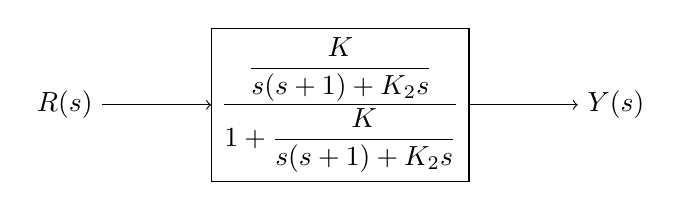
\begin{tikzpicture}[node distance = 3.5cm]
	\node[input] (r) {$ R(s) $};
	\node[block,right of=r] (G) {$ \dfrac{\dfrac{K}{s(s+1)+K_2s}}{1+\dfrac{K}{s(s+1)+K_2s}} $};
	\node[output,right of=G] (y) {$ Y(s) $};
	\draw[->] (r) -- (G);
	\draw[->] (G) -- (y);
	\end{tikzpicture}
\end{center}
Simplify the transfer function
\begin{center}
	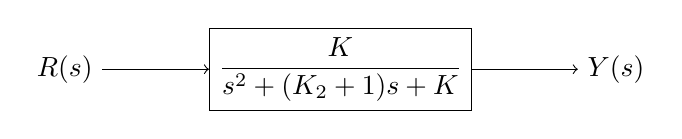
\begin{tikzpicture}[node distance = 3.5cm]
	\node[input] (r) {$ R(s) $};
	\node[block,right of=r] (G) {$ \dfrac{K}{s^2+(K_2+1)s+K}$};
	\node[output,right of=G] (y) {$ Y(s) $};
	\draw[->] (r) -- (G);
	\draw[->] (G) -- (y);
	\end{tikzpicture}
\end{center}

\section*{Block Diagram Manipulation}
Let's go over a few ways to move blocks around in a block diagram.
\subsection*{Moving a block across a summing junction}
Moving backwards:
\begin{center}
	\begin{tikzpicture}[node distance = 1.75cm]
		\node[input] (r) {$ R(s) $};
		\node[sum,right of=r] (sum) {$ \Sigma $};		
		\node[input,below of=sum] (x) {$ X(s) $};
		\node[block,right of=sum] (g) {$ G(s) $};
		\node[output,right of=g] (y) {$ C(s) $};
		\draw[->] (r) -- node[pos=0.9,above] {$+$} (sum);
		\draw[->] (x) -- node[pos=0.9,left] {$-$} (sum);
		\draw[->] (sum) -- (g);
		\draw[->] (g) -- (y);
		\node[right of=y,node distance = 1.375cm]  {$ \equiv $};
		
	\begin{scope}[shift={(8cm,0cm)}]
		\node[input] (r) {$ R(s) $};
		\node[block,right of=r] (g1) {$ G(s) $};
		\node[sum,right of=g1] (sum) {$ \Sigma $};
		\node[block,below of=sum] (g2) {$ G(s) $};		
		\node[input,below of=g2] (x) {$ X(s) $};
		\node[output,right of=sum] (y) {$ C(s) $};
		\draw[->] (r) -- (g1);
		\draw[->] (g1) -- node[pos=0.9,above] {$+$} (sum);
		\draw[->] (x) -- (g2);
		\draw[->] (g2) -- node[pos=0.9,left] {$-$} (sum);
		\draw[->] (sum) -- (y);
	\end{scope}
	\end{tikzpicture}
	\[ C(s) = (R(s)-X(s))G(s) \qquad \Leftrightarrow \qquad C(s) = R(s)G(s) - X(s)G(s) \]
\end{center}
Moving forwards:
\begin{center}
	\begin{tikzpicture}[node distance = 1.75cm]
	\node[input] (r) {$ R(s) $};
	\node[block,right of=r] (g) {$ G(s) $};
	\node[sum,right of=g] (sum) {$ \Sigma $};		
	\node[input,below of=sum] (x) {$ X(s) $};
	\node[output,right of=sum] (y) {$ C(s) $};
	\draw[->] (r) -- (g);
	\draw[->] (g) --node[pos=0.9,above] {$+$} (sum);
	\draw[->] (x) -- node[pos=0.9,left] {$-$} (sum);
	\draw[->] (sum) -- (y);
	\node[right of=y,node distance = 1.375cm]  {$ \equiv $};
	
	\begin{scope}[shift={(8cm,0cm)}]
	\node[input] (r) {$ R(s) $};
	\node[sum,right of=r] (sum) {$ \Sigma $};
	\node[block,below of=sum] (gi) {$ 1/G(s) $};		
	\node[input,below of=gi] (x) {$ X(s) $};
	\node[block,right of=sum] (g) {$ G(s) $};
	\node[output,right of=g] (y) {$ C(s) $};
	\draw[->] (r) -- node[pos=0.9,above] {$+$} (sum);
	\draw[->] (x) -- (gi);
	\draw[->] (gi) -- node[pos=0.9,left] {$-$} (sum);
	\draw[->] (sum) -- (g);
	\draw[->] (g) -- (y);
	\end{scope}
	\end{tikzpicture}
	\[ C(s) = R(s)G(s) - X(s) \qquad \Leftrightarrow \qquad C(s) = \left(R(s) - \dfrac{X(s)}{G(s)}\right)G(s) \]
\end{center}

\subsection*{Combining summing junctions}
Summing junctions can be combined together as follows:
\begin{center}
	\begin{tikzpicture}[node distance = 1.75cm]
	\node[input] (a) {$ A(s) $};
	\node[sum,right of=a] (sum1) {$ \Sigma $};		
	\node[input,below of=sum1] (b) {$ B(s) $};
	\node[sum,right of=sum1] (sum2) {$ \Sigma $};		
	\node[input,below of=sum2] (c) {$ C(s) $};
	\node[output,right of=sum2] (y) {$ Y(s) $};
	\draw[->] (a) -- node[pos=0.9,above] {$+$} (sum1);
	\draw[->] (b) -- node[pos=0.9,left] {$+$} (sum1);
	\draw[->] (c) -- node[pos=0.9,left] {$+$} (sum2);
	\draw[->] (sum1) -- (sum2);
	\draw[->] (sum2) -- (y);
	\node[right of=y,node distance = 1.375cm]  {$ \equiv $};
	
	\begin{scope}[shift={(8cm,0cm)}]
		\node[input] (a) {$ A(s) $};
		\node[sum,right of=r] (sum) {$ \Sigma $};		
		\node[input,below of=sum] (c) {$ C(s) $};
		\node[input,below left of=sum] (b) {$ B(s) $};
		\node[output,right of=sum] (y) {$ Y(s) $};
		\draw[->] (a) -- node[pos=0.9,above] {$+$} (sum);
		\draw[->] (c) -- node[pos=0.9,left] {$+$} (sum);
		\draw[->] (b) -- node[pos=0.9,above left] {$+$} (sum);
		\draw[->] (sum) -- (y);
	\end{scope}
	\end{tikzpicture}
\end{center}

\exmp
\begin{center}
	\begin{tikzpicture}[node distance = 1.5cm]
	\node[input] (r) {$ R(s) $};
	\node[sum,right of=r] (sum1) {$ \Sigma $};
	\node[waypoint,right of=sum1] (wp1) {};
	\node[block,right of=wp1] (G1) {$ G_1 $};
	\node[waypoint,above of=G1] (wp2) {};
	\node[sum,right of=G1] (sum2) {$ \Sigma $};
	\node[block,right of=sum2] (G2) {$ G_2 $};
	\node[waypoint,right of=G2] (wp3) {};
	\node[output,right of=wp3] (y) {$ Y(s) $};
	\node[waypoint,below of=G1] (wpb) {};
	
	\draw[->] (r) -- node[pos=0.9,above] {$ + $} (sum1);
	\draw[->] (sum1) -- (G1);
	\draw[->] (G1) -- node[pos=0.9,above] {$ - $} (sum2);
	\draw[->] (sum2) -- (G2);
	\draw[->] (G2) -- (y);
	\draw[->] (wp1) |- (wp2) -| node[pos=0.9,left] {$ + $} (sum2);
	\draw[->] (wp3) |- (wpb) -| node[pos=0.9,left] {$ - $}  (sum1);
	\end{tikzpicture}
\end{center}
Move $ G_2 $ behind the summing junction.
\begin{center}
	\begin{tikzpicture}[node distance = 1.5cm]
	\node[input] (r) {$ R(s) $};
	\node[sum,right of=r] (sum1) {$ \Sigma $};
	\node[waypoint,right of=sum1] (wp1) {};
	\node[block,right of=wp1] (G1) {$ G_1 $};
	\node[block,right of=G1] (G2) {$ G_2 $};
	\node[block,above of=G2] (wp2) {$ G_2 $};
	\node[sum,right of=G2] (sum2) {$ \Sigma $};
	\node[waypoint,right of=sum2] (wp3) {};
	\node[output,right of=wp3] (y) {$ Y(s) $};
	\node[waypoint,below of=G1] (wpb) {};
	
	\draw[->] (r) -- node[pos=0.9,above] {$ + $} (sum1);
	\draw[->] (sum1) -- (G1);
	\draw[->] (G1) -- (G2);
	\draw[->] (G2) -- node[pos=0.9,above] {$ - $}  (sum2);
	\draw[->] (sum2) -- (y);
	\draw[->] (wp1) |- (wp2);
	\draw[->] (wp2) -| node[pos=0.9,left] {$ + $} (sum2);
	\draw[->] (wp3) |- (wpb) -| node[pos=0.9,left] {$ - $}  (sum1);
	\end{tikzpicture}
\end{center}
Combine the parallel form:
\begin{center}
	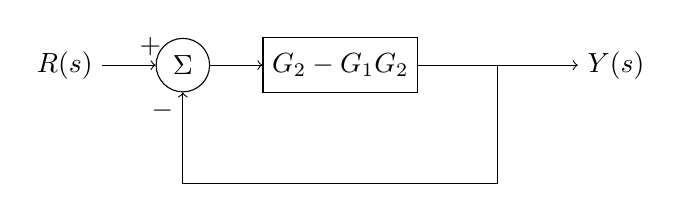
\begin{tikzpicture}[node distance = 1.5cm]
	\node[input] (r) {$ R(s) $};
	\node[sum,right of=r] (sum1) {$ \Sigma $};
	\node[block,right of=sum1,node distance = 2cm] (G1) {$ G_2-G_1G_2 $};
	\node[waypoint,right of=G1,node distance = 2cm] (wp3) {};
	\node[output,right of=wp3] (y) {$ Y(s) $};
	\node[waypoint,below of=G1] (wpb) {};
	
	\draw[->] (r) -- node[pos=0.9,above] {$ + $} (sum1);
	\draw[->] (sum1) -- (G1);
	\draw[->] (G1) -- (y);
	\draw[->] (wp3) |- (wpb) -| node[pos=0.9,left] {$ - $}  (sum1);
	\end{tikzpicture}
\end{center}
Reduce the feedback loop.
\begin{center}
	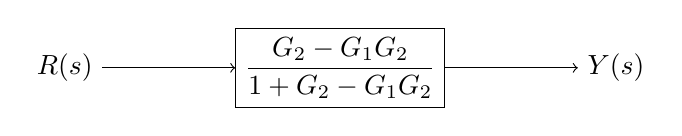
\begin{tikzpicture}[node distance = 3.5cm]
	\node[input] (r) {$ R(s) $};
	\node[block,right of=r] (G) {$ \dfrac{G_2-G_1G_2}{1+G_2-G_1G_2}$};
	\node[output,right of=G] (y) {$ Y(s) $};
	\draw[->] (r) -- (G);
	\draw[->] (G) -- (y);
	\end{tikzpicture}
\end{center}
\end{document}

